\clearpage
\thispagestyle{empty}

\vspace*{\fill}
\phantomsection
\addcontentsline{toc}{chapter}{Appendices}
\begin{center}
{\Huge\bfseries Appendices}
\end{center}
\vspace*{\fill}

\clearpage

\chapter{Probability and Expectation}

\section{Linearity of Expectation}
\label{linearity_of_expectation}
\noindent For any random variables $X_1,X_2,\dots,X_n$ (not necessarily independent),
\[
\mathbb{E}\left[\sum_{i=1}^n X_i\right]=\sum_{i=1}^n \mathbb{E}[X_i].
\]

\noindent\textbf{This holds regardless of dependence between variables.}
\section{Union Bound}
\label{union_bound}
For any events $A_1,A_2,\dots,A_n$,
\[
\Pr\left(\bigcup_{i=1}^n A_i\right)\le \sum_{i=1}^n \Pr(A_i).
\]

\noindent This is often used to upper bound the probability that at least one “bad event” occurs.

\section{Independence of Expectation}
\label{independence_of_expectation}
If $X$ and $Y$ are independent random variables, then
\[
\mathbb{E}[XY]=\mathbb{E}[X]\cdot \mathbb{E}[Y]
\]

\section{Variance}

\noindent For a random variable $X$, define the variance of $X$ as
\[
\mathrm{Var}(X)=\mathbb{E}[X^2]-\left(\mathbb{E}[X]\right)^2
\]

\vspace{1.5em}

\noindent For any two random variables $X$ and $Y$,
\[
\mathrm{Var}(X+Y)=\mathrm{Var}(X)+\mathrm{Var}(Y)+2\,\mathrm{Cov}(X,Y) \hspace{1em}(\text{where }
\mathrm{Cov}(X,Y)=\mathbb{E}[XY]-\mathbb{E}[X]\mathbb{E}[Y])
\]

\noindent If $X$ and $Y$ are independent, then $\mathrm{Cov}(X,Y)=0$, so
\[
\mathrm{Var}(X+Y)=\mathrm{Var}(X)+\mathrm{Var}(Y)
\]

\noindent More generally, for any collection $X_1,\dots,X_n$,
\[
\mathrm{Var}\left(\sum_{i=1}^n X_i\right)
=
\sum_{i=1}^n \mathrm{Var}(X_i)
+
2\sum_{1\le i<j\le n}\mathrm{Cov}(X_i,X_j).
\]

\section{Indicator Variables}
\label{indicator_variables}
\noindent For an event $A$, define the indicator random variable
\[
I_A=
\begin{cases}
1 & \text{if } A \text{ occurs},\\
0 & \text{otherwise}.
\end{cases}
\]
\vspace{0.3em}
\[
\implies
\mathbb{E}[I_A]=\Pr(A)
\]

\chapter{Inequalities}
\section{Exponential Inequality}
\label{exp_inequality}

\begin{center}
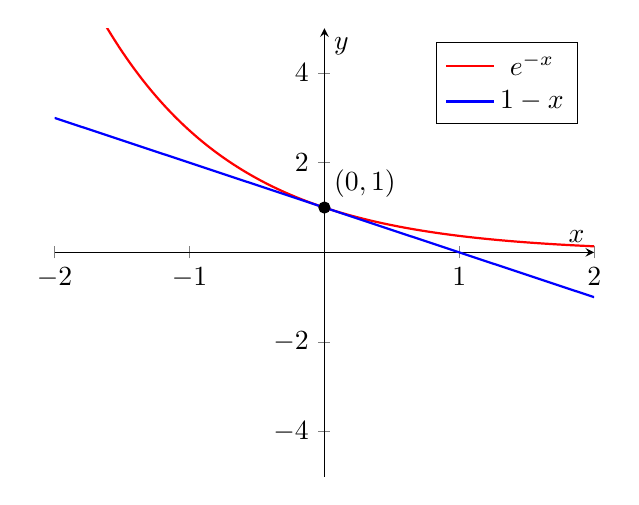
\begin{tikzpicture}
\begin{axis}[
    xmin=-2,xmax=2,
    ymin=-5,ymax=5,
    axis lines=middle,
    xlabel={$x$},
    ylabel={$y$},
    legend pos=north east
]
\addplot[red,thick,domain=-2:2,samples=200] {exp(-x)};
\addlegendentry{$e^{-x}$}

\addplot[blue,thick,domain=-2:2,samples=200] {1-x};
\addlegendentry{$1-x$}

\addplot[
    only marks,
    mark=*,
    mark size=2pt
]
coordinates {(0,1)};
\node[above right] at (axis cs:0,1) {$(0,1)$};
\end{axis}
\end{tikzpicture}
\end{center}
\vspace{-1em}
\[
1-x \le e^{-x} \hspace{0.5em} \forall \hspace{0.3em} x  \in \mathbb{R}
\implies
(1-x)^k \le e^{-kx} \hspace{0.5em} \forall \hspace{0.3em} k \in \mathbb{N}, x \in \mathbb{R}
\]


\section{Jensen’s Inequality}
\label{jensen}
For a concave-up function \(f\) and random variable \(X\),
\[
f(\mathbb{E}[X]) \le \mathbb{E}[f(X)]
\]

\noindent Another form of Jensen’s inequality is for a convex function \(f\) and real numbers \(x_1, x_2, \dots, x_n\), 
\[
f(\frac{1}{n}\sum_{i=1}^n x_i) \le \frac{1}{n}\sum_{i=1}^n f(x_i)
\iff
f(x_{avg}) \le y_{avg}
\]

\begin{center}
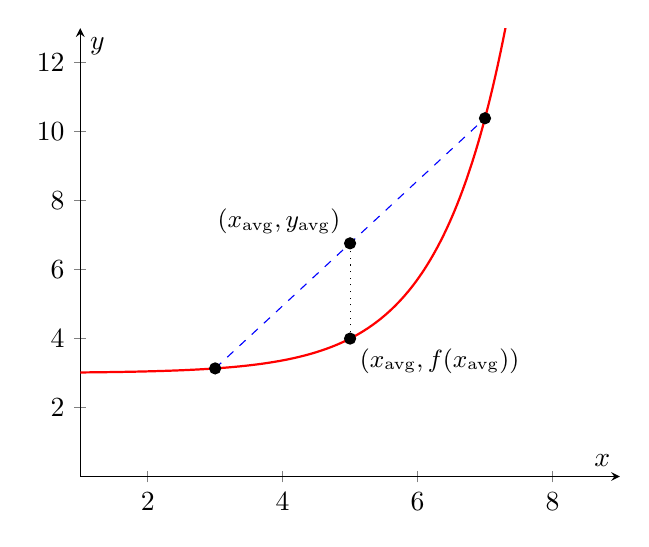
\begin{tikzpicture}
\begin{axis}[
    xmin=1,xmax=9,
    ymin=0,ymax=13,
    axis lines=middle,
    xlabel={$x$},
    ylabel={$y$},
    samples=200
]

\addplot[red,thick,domain=1:9] {exp(x-5)+3};

% endpoints
\addplot[only marks,mark=*,mark size=2pt]
coordinates {
(3,{exp(-2)+3})
(7,{exp(2)+3})
};

% chord
\addplot[blue,dashed]
coordinates {
(3,{exp(-2)+3})
(7,{exp(2)+3})
};

% midpoint on curve
\addplot[only marks,mark=*,mark size=2pt]
coordinates {(5,{exp(0)+3})};

\node[below right,font=\small] at (axis cs:5,4)
{$(x_{\mathrm{avg}},f(x_{\mathrm{avg}}))$};

% midpoint of chord
\pgfmathsetmacro{\yavg}{(exp(-2)+exp(2))/2}

\addplot[only marks,mark=*,mark size=2pt]
coordinates {(5,\yavg+3)};

\node[above left,font=\small] at (axis cs:5,\yavg+3)
{$(x_{\mathrm{avg}},y_{\mathrm{avg}})$};

% vertical segment showing the gap
\draw[dotted]
(axis cs:5,4)
--
(axis cs:5,\yavg+3);

\end{axis}
\end{tikzpicture}
\end{center}

\noindent For concave-down functions, the inequality is reversed, i.e. \(f(x_{avg}) \ge y_{avg}\).

\begin{center}
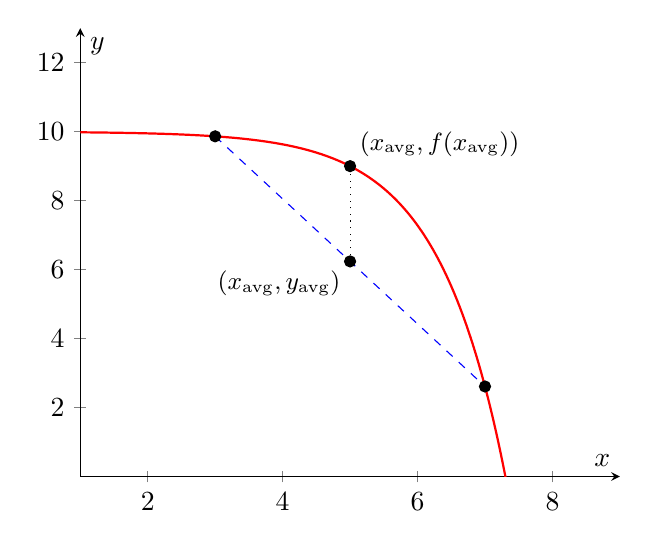
\begin{tikzpicture}
\begin{axis}[
    xmin=1,xmax=9,
    ymin=0,ymax=13,
    axis lines=middle,
    xlabel={$x$},
    ylabel={$y$},
    samples=200
]

\addplot[red,thick,domain=1:9] {10-exp(x-5)};

% endpoints
\addplot[only marks,mark=*,mark size=2pt]
coordinates {
(3,{10-exp(-2)})
(7,{10-exp(2)})
};

% chord
\addplot[blue,dashed]
coordinates {
(3,{10-exp(-2)})
(7,{10-exp(2)})
};

% midpoint on curve
\addplot[only marks,mark=*,mark size=2pt]
coordinates {(5,{10-exp(0)})};

\node[above right,font=\small] at (axis cs:5,9)
{$(x_{\mathrm{avg}},f(x_{\mathrm{avg}}))$};

% midpoint of chord
\pgfmathsetmacro{\yavg}{(10-exp(-2)+10-exp(2))/2}

\addplot[only marks,mark=*,mark size=2pt]
coordinates {(5,\yavg)};

\node[below left,font=\small] at (axis cs:5,\yavg)
{$(x_{\mathrm{avg}},y_{\mathrm{avg}})$};

% vertical segment showing the gap
\draw[dotted]
(axis cs:5,\yavg)
--
(axis cs:5,9);

\end{axis}
\end{tikzpicture}
\end{center}

\section{Markov's Inequality}
\label{markov_inequality}

\noindent Let \(X\) be a non-negative random variable and let \(a>0\). Then

\[
\Pr(X\ge a)
\le
\frac{\mathbb E[X]}{a}
\]
\subsection*{Proof}

\noindent Define the indicator variable $I$ as 
\[
I=
\begin{cases}
1 & \text{if } X\ge a,\\
0 & \text{otherwise}.
\end{cases}
\]

\noindent Then \(X\ge aI\) follows by definition! Taking expectations,

\[
\mathbb E[X]
\ge
a\,\mathbb E[I]
=
a\,\Pr(X\ge a)
\implies
\Pr(X\ge a)
\le
\frac{\mathbb E[X]}{a}
\]

\vspace{0.5em}
\noindent An equivalent and useful form is \(Pr(X\ge c\,\mathbb E[X])\le \frac{1}{c}\)


\chapter{Discrete Mathematics}

\section{Pigeonhole Principle}
\label{pigeonhole_principle}

Let \(a_1,a_2,\dots,a_n\) be non-negative real numbers and let
\[
S=\sum_{i=1}^{n}a_i,\hspace{0.5em} \text{then there \emph{exists} an $i$ such that }a_i \ge \frac{S}{n}
\]

This simply states that at least one value is at least the average value.

\subsection*{Proof by Contradiction}

If every \(a_i < \frac{S}{n}\), then summing over all \(i\) gives
\[
\sum_{i=1}^{n} a_i < S
\]
which is a contradiction.

\section{Graph Theory}

A graph $G$ is an ordered pair $(V,E)$ where \(V\) is a set of vertices 
and \(E\subseteq \{\{u,v\}\mid u,v\in V,\ u\neq v\}\) is a set of edges.
$|E|$ is usually denoted by \(m\) and $|V|$ is usually denoted by \(n\).
\subsection*{Degree}

For a vertex \(v\in V\), the degree \(d(v)\) is the number of edges which have \(v\) as an endpoint. 
Equivalently, \(d(v)\) is the number of neighbours of \(v\).\\

\noindent Given n is the number of vertices, the average degree 
of a graph is
\[
d=\frac{1}{n}\left(\sum_{v\in V} d(v)\right)=\frac{2m}{n}
\]

\subsection*{Bipartite Graph}

A graph \(G=(V,E)\) is bipartite if the vertex set \(V\) can be partitioned into two disjoint sets \(L\) and \(R\) such that
\[
V=L\cup R,\quad L\cap R=\emptyset
\]
and every edge connects a vertex in \(L\) to a vertex in \(R\). That is, there are no edges with both endpoints in the same set.

\subsection*{Subgraph}
A subgraph of a graph $(V,E)$ is a pair of sets $(V',E')$ where \(V'\subseteq V\) and \(E'\subseteq E\) with the 
additional condition that the subgraph must be a valid graph!

\chapter{Linear Algebra}

\section{Vector Spaces}
\label{vector_spaces}
Let \(\mathbb F\) be a field. A vector space over \(\mathbb F\) is a set \(V\)
equipped with vector addition and scalar multiplication satisfying the usual
axioms:

\begin{itemize}
\item closure under addition and scalar multiplication,
\item associativity and commutativity of addition,
\item existence of a zero vector,
\item existence of additive inverses,
\item distributive properties,
\item compatibility of scalar multiplication.
\end{itemize}

An example of a common vector space is the set of \(n\)-tuples of elements from \(\mathbb F\),
\[
\mathbb F^n
=
\{(x_1,x_2,\dots,x_n):x_i\in\mathbb F\}
\]

\vspace{0.4em}
Common choices for the field \(\mathbb F\) include the real numbers 
\(\mathbb R\) or the integers \(\mathbb Z\) with the usual addition and multiplication, 
and the finite field \(\mathbb F_p\) where \(p\) is a prime with addition and multiplication modulo \(p\).

\section{Subspaces}
\label{subspaces}
A subset \(W\subseteq V\) is called a subspace of the vector space \(V\) if

\begin{enumerate}
\item \(0\in W\)
\item for all \(u,v\in W\), we have \(u+v\in W\)
\item for all \(u\in W\) and \(\alpha\in\mathbb F\), we have
      \(\alpha u\in W\)
\end{enumerate}

\section{Dimension of a Subspace}
\label{dimension}
A collection of vectors $v_1,v_2,\dots,v_k$ is called a basis of a subspace \(W\) if

\begin{itemize}
\item the vectors are linearly independent
\item any vector in W is a linear combination of the vectors
\end{itemize}

The number of vectors in any basis of \(W\) is called the dimension of \(W\)
and is denoted by $\dim(W)$.

\section{The Nullspace}
\label{nullspace}
Let $M\in\mathbb F^{m\times n}$.
The nullspace of \(M\) is defined by

\[
\mathcal N(M)
=
\{x\in\mathbb F^n : Mx=0\}.
\]

\vspace{0.4em}
\noindent The nullspace is also called the \emph{kernel} of \(M\), and we write
\[
\ker(M)=\mathcal N(M).
\]
\noindent The nullspace of a matrix is a subspace of \(\mathbb F^n\).


\section{Nullity and Rank}
\label{nullity_and_rank}
Since the nullspace is a subspace, it has a well-defined dimension.\\


\noindent Define $\operatorname{nullity}(M)=\dim(\ker(M))$.\\


\noindent The rank of \(M\), denoted $\operatorname{rank}(M)$ is the dimension of the 
column space or row space of \(M\), equivalently the maximum number
of linearly independent columns or rows of \(M\).
\section{The Rank--Nullity Theorem}
\label{rank_nullity}
One of the fundamental results of linear algebra is the rank--nullity theorem.

\paragraph{Theorem (Rank--Nullity).}
For every matrix $M\in\mathbb F^{m\times n}$, we have

\[
\operatorname{rank}(M)
+
\operatorname{nullity}(M)
=
n.
\]
\vspace{0.4em}
An immediate consequence is that if \(M\neq0\), then

\[
\operatorname{rank}(M)\ge1,
\implies
\operatorname{nullity}(M)\le n-1.
\]



